\documentclass[letterpaper]{sig-alternate-05-2015}


%~~~~~~~~~~~~~~~~~~~~~~~~~~~~~~~~~~~~~~~~~~~~~~~~~~~~~~~~~~~~~~~~~~~~~~~~~~~~~~~~~~~~~~~~~~~~~~~~~~~~~~~

\usepackage{graphicx}
\usepackage[hidelinks]{hyperref} %[hidelinks] to hide hyperlinks
\usepackage[utf8]{inputenc}
\usepackage[normalem]{ulem}


%----------------------------------------------------------------------------------

% rename autorefnames
\def\sectionautorefname{Section}
\def\subsectionautorefname{Section}
\def\subsubsectionautorefname{Section}
\def\figureautorefname{Figure}
\def\tableautorefname{Table}

\usepackage{units}
\usepackage{siunitx}
\DeclareSIUnit\wn{\raiseto{-1}\cm}
\sisetup{
range-phrase = --,
range-units = single,
list-units = single,
product-units = single,
list-final-separator = {, and },
}


\usepackage{glossaries}
\makeglossaries
\newacronym{IoT}{IoT}{Internet of Things}
\newacronym{NFC}{NFC}{Near Field Communications}
\newacronym{RFID}{RFID}{Radio Frequency Identification}
\usepackage{notoccite}

\sloppy

%~~~~~~~~~~~~~~~~~~~~~~~~~~~~~~~~~~~~~~~~~~~~~~~~~~~~~~~~~~~~~~~~~~~~~~~~~~~~~~~~~~~~~~~~~~~~~~~~~~~~~~~


\begin{document}

\doi{XXXX}
\isbn{XXXX}

\title{Gesture-Based Peer-to-Peer Pairing Authentication for Assymmetric \glsentrylong{IoT} Devices}

\numberofauthors{3} 
\author{
% 1st. author
\alignauthor
Joe Chen\\
       \email{joe.chen@rice.edu}
 % 2nd author
 \alignauthor
Zilong Liao\\
       \email{zl15@rice.edu}
 % 3rd author
\alignauthor
Heng-Yi Lin\\
       \email{henry.hy.lin@rice.edu}
}

\maketitle
%\begin{abstract}
%\input{chapters/abstract}
%\end{abstract}

%%!TEX root = ../iotpaper.tex

\section{Introduction}
\label{sec:Introduction}

In an \gls{IoT} environment, mobile devices may need to pair or authenticate themselves to other devices. However, unlike the traditional internet, an \gls{IoT} environment does not typically have a centralized certificate authority, making it difficult for one device to determine if another device is authentic. Furthermore, these \gls{IoT} devices are often resource-constrained, meaning traditional cryptographic defenses that support confidentiality, integrity, and authenticity difficult to implement \cite{cisco:iot-pf,authmodels}.

One potential solution to this problem is to use biometrics---especially motion and gestures---in order to validate the identity of the device. Prior work has shown that impostors has a low probability of imitating a gesture calibrated to another person successfully \cite{Casanova}. Furthermore, motion recognition is suitable for \gls{IoT} systems which feature small sensors and low powered devices because motion recognition can achieve high accuracy with just an accelerometer \cite{RuizeXu}. 

Some prior work have looked at motion sensor data fusion across different devices to detect pairing, for example detecting device collision when tiling two tablets together \cite{SyncGes}. Existing work in gesture recognition and event detection focuses on gestures on the same device or similar devices (e.g. two tablets, gestures on a Wiimote \cite{LiuuWave}). However, pairing in an \gls{IoT} environment is usually needed for two asymmetric devices with different types of hardware sensors (e.g. a smartwatch with a smartphone).

In this project, we analyze the use of gestures as a biometric for peer-to-peer authentication in an \gls{IoT} scenario, where sensor devices are asymmetric. 

\section{Attack \& Defense Models}
\label{sec:Attacks}

Our project analyzes the following three key defense models for authentication.

\begin{itemize}
\item \emph{Model 1:} This system model contains three entities: a legitimate prover, a verifier, and an attacker. The legitimate prover is non-malicious and wants to pair with the verifier. Both the legitimate prover and the verifier are owned by the same person (e.g. a smartphone and a smartwatch). However, the attacker is a malicious prover and wants to also pair with the verifier. To distinguish between the attacker and legitimate prover, the verifier uses gesture recognition to distinguish between the two parties. 

\begin{figure}[!tb]
\centering
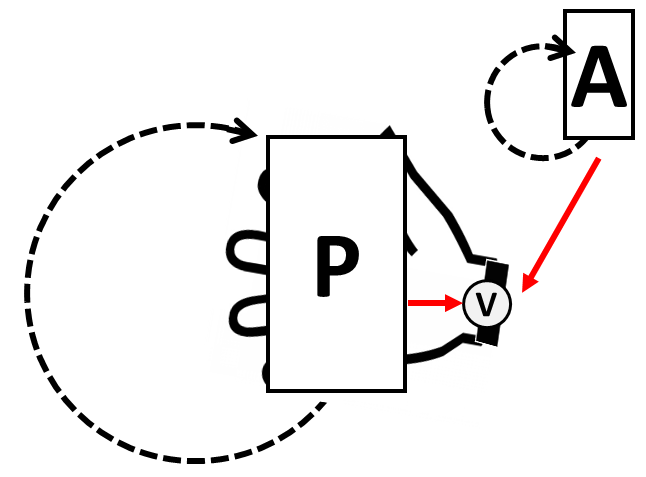
\includegraphics[width=0.65 \linewidth]{./figures/model1.png}
\caption{System model for defense model 1. The verifier (V) and the prover (P) are synchronized in motion. The attacker (A) must try to mimic the motion of the verifier in order to trick the system.}
\label{fig:Model1}
\end{figure}

Since the legitimate prover and verifier are owned by the same person, the user performs any generic gesture while holding both devices as shown in \autoref{fig:Model1}. Accelerometer data is used to read the gesture, and a matching gesture authenticates the prover.

In contrast, the attacker must mimic the gesture of the verifier in order to trick the verifier. Our hypothesis is that we can keep false negatives (rejecting legitimate provers) and false positives (accepting attackers) to less than 10\%. This is modest compared to existing works due to the hardware asymmetry.  

\item \emph{Model 2:} This system model contains the same three entities as in Model 1. In this model, the verifier has previously calibrated a single secret gesture with the user that is needed to pair with the device as shown in \autoref{fig:Model2}. Devices that want to pair with the verifier must produce accelerometer data that matches this gesture with no prior knowledge about the gesture. Since this gesture is a predefined secret, only the prover needs to collect accelerometer data during the proof of authenticity.

\begin{figure}[!tb]
\centering
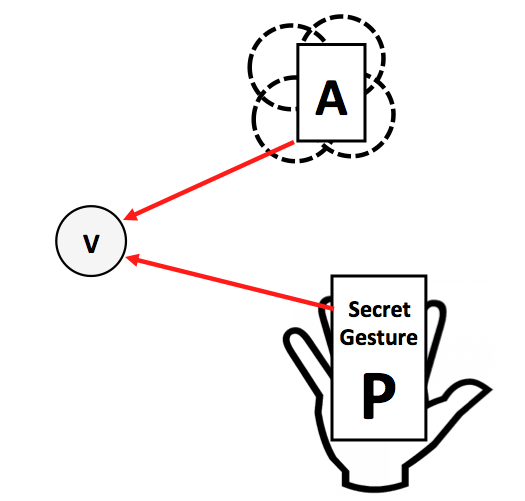
\includegraphics[width=0.6 \linewidth]{./figures/model2.png}
\caption{System model for defense model 2. The verifier (V) and the prover (P) are not synchronized in motion, and the verifier has previously established a secret gesture for pairing. The attacker (A) can brute force a gesture if it has no knowledge of the secret gesture, or it may imitate a gesture that it sees that a legitimate prover used.}
\label{fig:Model2}
\end{figure}

An attacker may try to trick this model in the following two ways. First, if no information about the secret gesture has been leaked to the attacker, it will attempt a brute force attack and attempt several common gesture shapes, such as a circle, line, or even just shaking the device. Second, an attacker may learn information about which gesture is the secret gesture by watching a legitimate prover validate themselves to the verifier. These visual clues then reveal what the actual gesture is, and the attacker scenario reduces to the same as in Model 1. 

For the second attack, we hypothesize that we will again achieve less than 10\% false negatives for legitimate provers. However, we hypothesize 0\% false positives for attackers if the secret gesture is not within the library of brute force attempts (i.e. the gesture recognition algorithm works). 

\item \emph{Model 3:} The final model once again contains the same three entities as the prior models. Although similar to Model 2, this model establishes a pre-defined library of gestures at the verifier previously calibrated by the user. During the pairing process, the verifier will challenge the prover to a subset of the gesture library. As shown in \autoref{fig:Model3}, the verifier sends visual prompts about what the gestures should be during the challenge process (i.e. the library of gestures is public). However, to trick the system, an attacker must produce the gesture in the same way as the intended user. 

\begin{figure}[!tb]
\centering
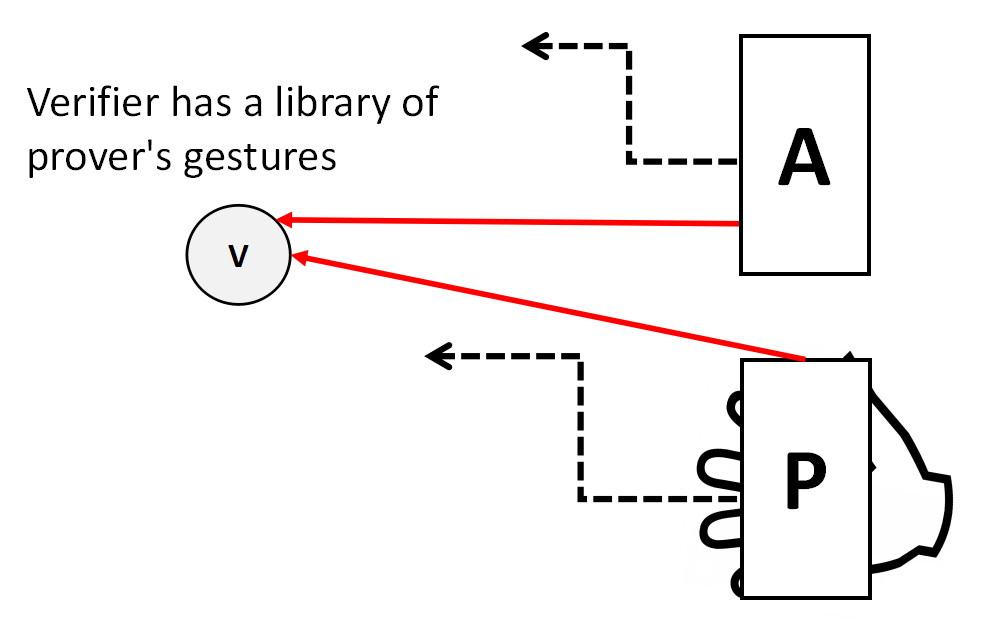
\includegraphics[width=0.65 \linewidth]{./figures/model3.png}
\caption{System model for defense model 3. The verifier (V) and the prover (P) are not synchronized in motion, and the verifier challenges the prover with a series of gestures in its pre-calibrated library. The attacker (A) receives the same prompts, but must mimic what the prover would do for each gesture.}
\label{fig:Model3}
\end{figure}

We hypothesize that there is a inverse correlation between number of gesture challenges and number of false positives (i.e. more challenges reduces the success of an attacker. However, we also hypothesize there is a direct correlation between number of gesture challenges and number of false negatives (i.e. there are more opportunities for the user to fail). We seek to find a threshold that minimizes the number of false positives and false negatives in this model.

\end{itemize}


%%!TEX root = ../iotpaper.tex

\section{Lightweight Cryptography}
\label{sec:crypto}

While the conventional cryptography may have provided sufficient protection for the sensitive data and built robust foundation for various aspects of information security, modern cryptosystems based on them are not applicable to most cases in the \gls{IoT} Era. Most \gls{IoT} devices are resource-constrained that they typically have limited computing power, memory, and battery capacity. They may also be low-cost and small-sized. All these possible constraints make conventional strong cryptographic schemes, which require relatively high performance computing platform, practically or commercially infeasible \cite{cisco:iot-pf}. 

To overcome aforementioned limitations, research work and applications focus on lightweight cryptography, specified in ISO/IEC 29192-1 \cite{ISO29192-1:2012}, which is suitable for environments where may encounter any of the following limitations:
\begin{itemize}
\item chip area,
\item energy consumption,
\item program code size and RAM size,
\item communication bandwidth,
\item and execution time.
\end{itemize}

Lightweight cryptography is always coped with tradeoff among security, cost, and performance in varied implementations (\textquotedblleft Lightweight Ciphers," 2016)\footnote{In CryptoWiki. Accessed: 2016-02-18, from \url{http://cryptowiki.net/index.php?title=Lightweight_ciphers}}. According to a survey by Eisenbarth et. al. \cite{Eisenbarth:2007}, these implementation can be classified in two ways: software-oriented against hardware-oriented or symmetric against asymmetric. First, software-oriented implementations are used in areas where memory requirements and power consumption are main concerns, while hardware-oriented ones are implemented in scenarios where the chip size and number of clock cycles are primary consideration. Second, asymmetric cryptography are secure with more functionality but more demanding in memory, computing power, and power consumption compared with symmetric cryptography \cite{Tripathi:2014}.

Among various proposed lightweight cryptographic schemes, we enumerate existing standardized schemes under ISO/IEC 29192 standardization. Our objective for this project is to evaluate those schemes based on their performance, security level, and practical feasibility on the same platform.

In the following subsections, we briefly depict some differences between lightweight and conventional primitives, and introduce primitives which we intend to analyze. 

\subsection{Lightweight Symmetric Cryptography}

\subsubsection{Block Ciphers}

Unlike conventional block ciphers such as AES and Twofish, lightweight ciphers commonly have smaller key size and block size. As Bogdanov et. al. \cite{Cazorla:2013} has specified, they also tend to extremely simplify key schedule but have more required number of rounds due to the deeper dependence on elementary operations. 

Among proposed lightweight block cryptography, PRESENT \cite{Bogdanov:2007}, an ultra-lightweight block cipher based on S-P networks, and CLEFIA \cite{Shirai:2007}, a generalized Feistel-structured block cipher with Diffusion Switching Mechanism, has been adopted as the new international standards for lightweight cryptographic implementations under ISO/IEC 29192-2 \cite{ISO29192-2:2012}. 

\subsubsection{Stream Ciphers}

Because of the nature of stream ciphers, stream ciphers are of great use in processing unknown-length or varied-length data. Furthermore, they are generally more efficient than block ciphers that software-oriented ones take fewer CPU cycles and hardware-oriented ones require smaller chip area. These characteristics make them suitable for \gls{IoT} settings.

Among current lightweight stream ciphers, ISO/IEC 29192-3 \cite{ISO29192-3:2012} has specified the following two stream ciphers as international standards for lightweight stream ciphers: Trivium, a hardware-oriented stream cipher proposed by De Cannière and Preneel \cite{DeCanniere:2006} in eSTREAM project, which leverages an idea from the design principles of block ciphers to reduce linear correlations and provides flexibility between number of gates and speed of encryption; and Enocoro, a hardware-oriented stream cipher proposed by Watanabe et. al. \cite{Watanabe:2008}, which is efficient in both software and hardware implementation compared to eSTREAM hardware-oriented stream ciphers.

\subsubsection{Hash Functions}

In the \gls{IoT} era, low-cost \gls{RFID} tags are used extensively and they often rely on hash functions for encryption. According to Juels and Weis \cite{Juels:2005}, \gls{RFID} tags have only 2000 gates for security purpose. However, the conventional hash functions generally have more than 10000 gates that they are costly and exceed the security gate count budget. Therefore, lightweight hash functions are designed to mitigate gate counts that they can then fit into this scenario. Even though ISO/IEC 29192-5 is still under development, presented strong candidates of lightweight hardware-optimized hash functions including PHOTON (738GE\footnote{Gate Equivalence.}) and SPONGENT (865GE) both have significantly low gate count\footnote{Statistics from Lightweight Hash Functions. In CryptoLUX. Accessed: 2016-02-21, from \url{https://www.cryptolux.org/index.php/Lightweight_Hash_Functions}}.

\subsection{Lightweight Asymmetric Cryptography}

Asymmetric cryptography is widely known by its strength in securing the channel with an insecure medium and is used in various applications, but it comes with a price that it typically requires more in computational platform resources. In the context of the \gls{IoT}, its demanding characteristic may make it seem less practical. Nonetheless, recent research has proposed several lightweight mechanisms based on asymmetric techniques and some of them have been adopted as ISO/IEC 29192-4 \cite{ISO29192-4:2013} standards. These adopted lightweight mechanisms include: cryptoGPS \cite{Girault:2006}, an identification scheme based on discrete logarithm; ALIKE (previously called SPAKE) \cite{Coron:2010}, an authenticated key exchange protocol based on RSA (Rivest-Shamir-Adleman) encryption; and an identity-based signature scheme proposed by Liu et. al. \cite{Liu:2010}.

%%!TEX root = ../iotpaper.tex

\section{Motion Authentication}
\label{sec:motionauth}

Biometrics is becoming increasingly easy to observe in commercial products. Biometric recognition is based on human physiological and/or behavioral characteristics \cite{Jain}. Fingerprint authentication, a typical example of physiological biometrics, is being applied to more and more smartphones since Apple embedded a fingerprint recognition module in iPhone. Behavioral biometrics utilizes human dynamic characteristics and has become a trend in biometrics. Some human dynamic characteristics can be used to recognize the genuineness of user correctly, such as prehension biometrics\cite{Drosou}. Similarly, motion recognition is suitable for \gls{IoT} systems which feature small sensors and low powered devices because motion recognition can achieve high accuracy with just an accelerometer \cite{RuizeXu}.

\subsection{A Possible Application}
Based on above analysis, therefore, one possible application of motion recognition is for pairing smartphone with IoT devices embedded with accelerometers. Pairing authentication is necessary because smartphone is one of the most popularly used device to control \gls{IoT} networks in today's market. We propose the following solution: the smartphone shows a specific personalized moving pattern that was defined by user previously and then the user needs to move the \gls{IoT} device in this pattern and the accelerometer data from the \gls{IoT} device is sent to the smartphone. The smartphone then compares the motion data with the existing database to check if the pattern is correct and is done by the same user with behavioral biometrics analysis. If so, the pairing succeeds. In this case, even though the smartphone is controlled by an attacker, the pairing cannot succeed. Conversely, in the opposite case, the \gls{IoT} device can ask the smartphone to perform a predefined motion and IoT device with stronger processor or connection to a server can determine if the motion data from the smartphone matches.  Also, if the \gls{IoT} is small enough, the user can hold both the \gls{IoT} device and the smartphone to perform a specific motion at the same time. Then both devices can just compare the motion data from the other device with its own. In this case, no database is needed.

\subsection{Feasibility}

As mentioned above, motion recognition with only accelerometer gives high accuracy, thus how to set up a biometric database to check if the motion is performed by correct user become the main concern of this solution. A feasible solution provided by Guerra et al. \cite{Casanova} is as the following. They let the user to invent their personal gesture and offer 7 samples to the database. Users give really different gestures, such as writing a word and drawing some symbol in the air. All these gestures are collect while holding a device with an accelerometers embedded. The result from Guerra et al. \cite{Casanova} shows that the impostors has a very low chance of imitating successfully. This method can be applied to the pairing between smartphone and \gls{IoT} devices. Smartphone can just show a hint of the gesture or even nothing to have a higher security level.

\subsection{Equipment and Algorithm}
Obviously, a smartphone and an additional device embedded with accelerometers that can connect with the smartphone in bluetooth or some other ways are needed for this solution. Other than these, an efficient recognition algorithm: uWave can be used in this solution, because this algorithm requires only one accelerometer and is proved by Jiayang et al. \cite{Liu:2009, LiuuWave} from Rice University that it well recognized personalized gestures.
%%!TEX root = ../iotpaper.tex

\section{Authentication Models}
\label{sec:otherauth}

In traditional networks over the internet, the certificate authority hosts validates sites as authentic. This system protects a user from thinking they are visiting one site (e.g. Amazon, Google, etc.) when they are actually visiting another site. However, this paradigm is not achievable in an \gls{IoT} environment because there is no certificate authority for every device in the environment. As a result, an \gls{IoT} network must rely on its own alternative methods to support peer-to-peer authentication.

In this project, we propose implementation and a security analysis of one of the existing security paradigms for peer-to-peer authentication listed in the following sections. In particular, we aim to simulate a reputation system and evaluate it under different environments and attackers. Our evaluation would be geared towards minimizing both false positives and false negatives when a node has to decide whether or not to trust a new node trying to authenticate itself.

In the remainder of this section, we discuss existing \gls{IoT} authentication methods in greater detail.

\subsection{Gateway Authentication}

One simple method of peer-to-peer authentication is the use of a gateway. In this method, the gateway (e.g. a smartphone) serves as a central authority and all \gls{IoT} devices (e.g. sensors, controllers, etc.) authenticate themselves to the gateway. The gateway then validates authentication individually. One form of gateway authentication was proposed in \cite{gatewayauth} where one party is inside the local \gls{IoT} network, and one device is outside the network. The gateway communicates with the external device using traditional security protocols (e.g. IPSec) and will rencrypt communication with the local device. In the Secure Gateway Application (SGA), the authors propose offloading heavy cryptographic primitives needed for authentication schemes to a central SGA server, allowing for a lightweight implementation on non-gateway devices \cite{Gateway2016}. A centralized gateway for authentication is also used as the cornerstone of the \gls{IoT} framework proposed in \cite{AuthZ}.

Gateway authentication produces a heavy traffic burden on the gateway itself and may bottleneck in systems with a dense deployment of \gls{IoT} devices. These gateways also become a critical point for security because a compromised gateway undermines the security of the entire network \cite{authmodels}. 

\subsection{Reputation System}

An alternative to gateway authentication is to instead offload the trust system into the peer-to-peer network itself. Leister et. al. propose a trust indicator model for \gls{IoT} devices. Based on observers already trusted in the network, a device calculates a priori trust to determine if it should trust the new party \cite{trustindicator}. Similarly, Chen et. al. use a fuzzy trust model as their reputation system. This model uses the observations of neighbors to calculate the reputation of a node using the following metrics: end-to-end packet forwarding ratio, energy consumption when delivering/receiving messages, and packet delivery ratio \cite{DongChen2011}. 

Although distributing this decision reduces the strain on the gateway, this reputation system weakens if a malicious device slips into the network \cite{authmodels}.

%!TEX root = ../iotpaper.tex

\section{Project Proposal}
\label{sec:Proposal}

In an \gls{IoT} environment, mobile devices may need to pair or authenticate themselves to other devices. However, unlike the traditional internet, an \gls{IoT} environment does not typically have a centralized certificate authority, making it difficult for one device to determine if another device is authentic. Furthermore, these \gls{IoT} devices are often resource-constrained, meaning traditional cryptographic defenses that support confidentiality, integrity, and authenticity difficult to implement \cite{cisco:iot-pf,authmodels}.

One potential solution to this problem is to use biometrics---especially motion and gestures---in order to validate the identity of the device. Prior work has shown that impostors has a very low probability of imitating a gesture calibrated to another person successfully \cite{Casanova}. Furthermore, motion recognition is suitable for \gls{IoT} systems which feature small sensors and low powered devices because motion recognition can achieve high accuracy with just an accelerometer \cite{RuizeXu}. 

Some prior work have looked at motion sensor data fusion across different devices to detect pairing, for example detecting device collision when tiling two tablets together \cite{SyncGes}. Existing work in gesture recognition and event detection focuses on gestures on the same device or similar devices (e.g. two tablets, gestures on a Wiimote \cite{LiuuWave}). However, pairing in an \gls{IoT} environment is usually needed for two asymmetric devices with different types of hardware sensors (e.g. a smartwatch with a smartphone).

In this project, we propose to analyze the use of gestures as a biometric for peer-to-peer authentication in an \gls{IoT} scenario, where sensor devices are asymmetric. 
Our project will analyze the following three key defense models for authentication.

\begin{itemize}
\item \emph{Model 1:} This system model contains three entities: a legitimate prover, a verifier, and an attacker. The legitimate prover is non-malicious and wants to pair with the verifier. Both the legitimate prover and the verifier are owned by the same person (e.g. a smartphone and a smartwatch). However, the attacker is a malicious prover and wants to also pair with the verifier. To distinguish between the attacker and legitimate prover, the verifier uses gesture recognition to distinguish between the two parties. 

\begin{figure}[!tb]
\centering
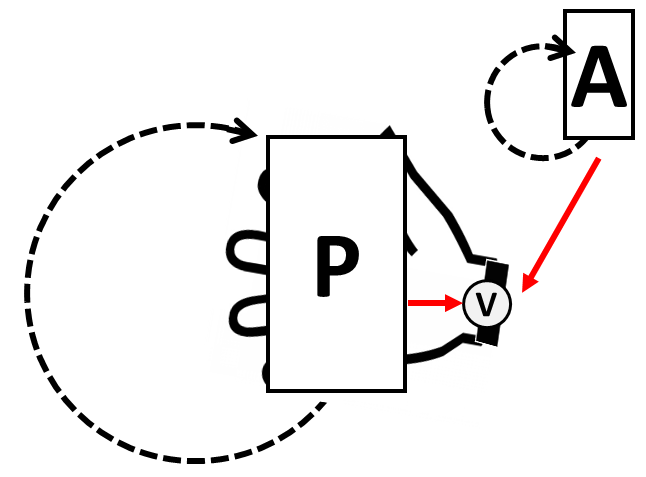
\includegraphics[width=0.65 \linewidth]{./figures/model1.png}
\caption{System model for defense model 1. The verifier (V) and the prover (P) are synchronized in motion. The attacker (A) must try to mimic the motion of the verifier in order to trick the system.}
\label{fig:Model1}
\end{figure}

Since the legitimate prover and verifier are owned by the same person, the user performs any generic gesture while holding both devices as shown in \autoref{fig:Model1}. Accelerometer data is used to read the gesture, and a matching gesture authenticates the prover.

In contrast, the attacker must mimic the gesture of the verifier in order to trick the verifier. Our hypothesis is that we can keep false negatives (rejecting legitimate provers) and false positives (accepting attackers) to less than 10\%. This is modest compared to existing works due to the hardware asymmetry.  

% To pair two devices together, the devices simultaneously measure the motion with the accelerometer. If the data matches, then the devices successfully pair. An attacker for this system tries to impersonate a gesture that the verifier is using.

\item \emph{Model 2:} This system model contains the same three entities as in Model 1. In this model, the verifier has previously calibrated a single secret gesture with the user that is needed to pair with the device as shown in \autoref{fig:Model2}. Devices that want to pair with the verifier must produce accelerometer data that matches this gesture with no prior knowledge about the gesture. Since this gesture is a predefined secret, only the prover needs to collect accelerometer data during the proof of authenticity.

\begin{figure}[!tb]
\centering
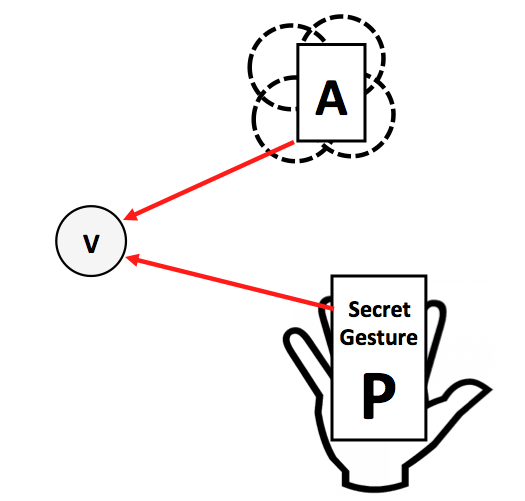
\includegraphics[width=0.6 \linewidth]{./figures/model2.png}
\caption{System model for defense model 2. The verifier (V) and the prover (P) are not synchronized in motion, and the verifier has previously established a secret gesture for pairing. The attacker (A) can brute force a gesture if it has no knowledge of the secret gesture, or it may imitate a gesture that it sees that a legitimate prover used.}
\label{fig:Model2}
\end{figure}

An attacker may try to trick this model in the following two ways. First, if no information about the secret gesture has been leaked to the attacker, it will attempt a brute force attack and attempt several common gesture shapes, such as a circle, line, or even just shaking the device. Second, an attacker may learn information about which gesture is the secret gesture by watching a legitimate prover validate themselves to the verifier. These visual clues then reveal what the actual gesture is, and the attacker scenario reduces to the same as in Model 1. 

For the first attack in the second model, we hypothesize that we will again achieve less than 10\% false negatives for legitimate provers. However, we hypothesize 0\% false positives for attackers if the secret gesture is not within the library of brute force attempts (i.e. the gesture recognition algorithm works). 

\item \emph{Model 3:} The final model one again contains the same three entities as the prior models. Although similar to Model 2, this model establishes a pre-defined library of gestures at the verifier previously calibrated by the user. During the pairing process, the verifier will challenge the prover to a subset of the gesture library. As shown in \autoref{fig:Model3}, the verifier sends visual prompts about what the gestures should be during the challenge process (i.e. the library of gestures is public). However, to trick the system, an attacker must produce the gesture in the same way as the intended user. 

\begin{figure}[!tb]
\centering
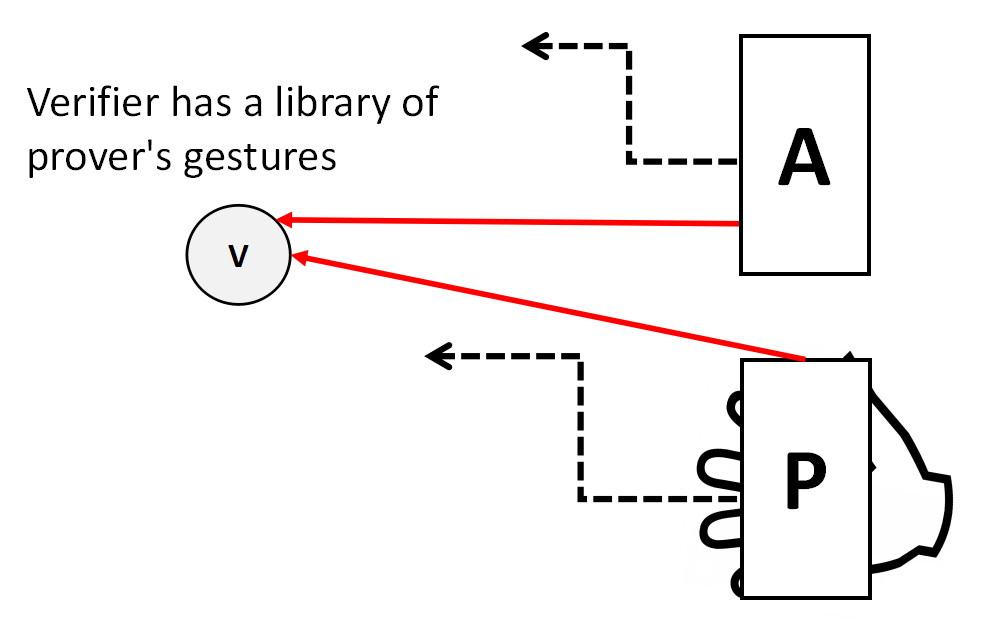
\includegraphics[width=0.65 \linewidth]{./figures/model3.png}
\caption{System model for defense model 3. The verifier (V) and the prover (P) are not synchronized in motion, and the verifier challenges the prover with a series of gestures in its pre-calibrated library. The attacker (A) receives the same prompts, but must mimic what the prover would do for each gesture.}
\label{fig:Model3}
\end{figure}

We hypothesize that there is a inverse correlation between number of gesture challenges and number of false positives (i.e. more challenges reduces the success of an attacker. However, we also hypothesize there is a direct correlation between number of gesture challenges and number of false negatives (i.e. there are more opportunities for the user to fail). We seek to find a threshold that minimizes the number of false positives and false negatives in this model.

%The verifier has a library of gestures previously calibrated by the user. To pair with the verifier, the prover must respond to the verifier's challenge. The verifier will send a gesture image/shape to the prover, and the prover must produce accelerometer data that matches the gesture data at the verifier. 

\end{itemize}


%!TEX root = ../iotpaper.tex

\subsection{Existing Tooling \& Research Platform}
\label{sec:Tooling}

We aim to use uWave \cite{Liu:2009, LiuuWave}, an algorithm developed at Rice, for gesture recognition during our security analysis. This algorithm is simple and efficient that even simple 16-bit microcontroller can do the computation. 

To test asymmetric pairing between different devices, we plan to use an android smartphone, an iPhone, and also another device with an accelerometer (the details of this \gls{IoT} style device is to be determined after discussion with people from uWave team). Ideally, we will test pairing across each of these 3 devices with a smartphone app.

%!TEX root = ../iotpaper.tex

\section{Progress}
\label{sec:Progress}

\subsection{Current Accomplishments}

\begin{itemize}
\item Successfully extracted accelerometer data from all three mobile devices
\item Basic gesture functionality of uWave converted to MATLAB programming environment.
\item Initial distance measurements between non-malicious and malicious provers for gesture recognition on a signle device.
\end{itemize}

\subsection{Future Milestones}

\begin{itemize}
\item \emph{April 6:} Rigorous Model 3 experiments completed. Scripting for Model 1 completed (remove axis/orientation bias).
\item \emph{April 13:} Rigorous Model 1 \& 2 testing completed. 
\item \emph{April 22:} Finalize project report/conduct follow up experiments. 
\item \emph{Final Exam Period:} Final project presentation
\end{itemize}

\subsection{Generalized Division of Labor}

\begin{itemize}
\item \emph{Joe:} Lead for MATLAB software development and wiimote integration.
\item \emph{Zilong:} Lead for Android software development. 
\item \emph{Heng-Yi:} Lead for iOS software development. 
\end{itemize}



%!TEX root = ../iotpaper.tex

\section{Related Work}
\label{sec:RelatedWork}

Our related work is divided into three key categories: (1) gesture recognition algorithms and implementations on a single accelerometer device, (2) device pairing via accelerometer data, and (3) other biometric recognition authentication techniques.

%!TEX root = ../iotpaper.tex

\subsection{Gesture \& Motion Recognition on a Single Device}

Several efficient gesture-recognition algorithms already exist. Jiayang et al. \cite{Liu:2009, LiuuWave} presented an algorithm called uWave that is based on a single accelerometer. uWave quantizes the acceleration data to reduce computational load and uses dynamic time warping(DTW) to measure similarities between two time series of accelerometer data. Template adaptation deals with gesture variation over the time. Ahmad and Shahrokh \cite{Ahmad:2010} also proposes a gesture recognition system that uses only one 3-axis accelerometer. The system temporally compresses the acceleration time series to filter out variations not intrinsic to the gesture itself and reduces the size of the acceleration signals for next step of dynamic time warping. Then, the system uses affinity propagation to find a good set of exemplars from all data points. Finally, they implemented compressive sensing to recognize a repetition of a gesture. 

For the best user experience, gesture recognition should be in real-time and easy to use. Instead of using a button to indicate start time and end time of a gesture motion, Zoltan \cite{Zoltan} proposes an automatic segmentation method and uses two classification algorithms: Hidden Markov Models(HMM) and Support Vector Machine to to give high accuracy. This system has great performance and low response time, thus a good model for \gls{IoT} devices.

Considering the quadratic time and space complexity with DTW algorithm and the need of larger training sets with HMM, Zhe Ji et al. \cite{Ji:2015} proposed a new algorithm which uses FastDTW instead of DTW and HMM. Their algorithm is divided into two part: preprocess and classification. In the preprocessing step, the raw data is first filtered by a series of low-pass filters and its amplitude is normalized. Then, it is resampled to a fixed length. After preprocessing the raw data, FastDTW, which has linear time and space complexity, is used to calculated the alignment between two time series. Their work shows that the performance drop is not necessary and is avoidable while replacing lightweight FastDTW to DTW for reducing computational demand.

%!TEX root = ../iotpaper.tex

\subsection{Device Pairing via Sensor Data}

In addition to recognition of a gesture, gesture-detection can also be used as a form of multifactor authentication to pair two separate devices together. Hinckley proposed one of the earlier forms of synchronous gesture authentication. By detecting an impulse when two tablets are pushed together, Hinckley pairs the two tablets, allowing the user to tile both devices together as one large screen \cite{SyncGes}. Vinteraction uses a combination of accelerometer and vibrator data to transmit private data between two devices in physical contact. The vibrations serve as the secret shared channel between the two devices \cite{vinteraction}. Mayrhofer et. al. have a user hold two mobile devices and shake randomly to establish a shared secret key. The shaking motion produces enough entropy to create a key that is difficult to predict \cite{ShakeWell}.

Jiang et. al. propose near-field vibration (NFV) to group multiple devices together at once. By propagating the vibrations of a smartphone through a table on which all group devices are placed, the smartphone can automatically pair with all of the devices in the group \cite{Jiang2016}. 

In a non-security based scenario, Duet explores combining sensor information for both a smartphone and a paired watch to create more sophisticated controls based on hand gestures \cite{Duet}. PickRing compares gyroscope data across a ring and a gyroscope to detect when a user picks up a smart device. However, the authors do not analyze the security of this approach against a malicious prover \cite{Wolf:2015}.

%!TEX root = ../iotpaper.tex

\subsection{Other Biometric Recognition Authentication Techniques}

Besides motion and gesture, various biometric characteristics could also be used for recognition as Jain et al. \cite{Jain} specified. These characteristics include: DNA, ear, face, facial thermogram, hand thermogram, hand vein, fingerprint, gait, hand geometry, iris, palmprint, retina, signature, and voice. In some applications, biometric traits are further exploited for machine-to-machine recognition authentication instead of conventional personal recognition.

One example of this idea is an authentication scheme based on heartbeat data (ECG) proposed by Rostami et al.\cite{Rostami:2013} It requires that the controller of implantable medical devices (IMDs) contacts the patient's body to control the IMD. Specifically, the controller can only gain access to IMDs if the ECG readings on the both devices are approximately the same.  
 
Furthermore, a patent \cite{Apple:2014} submitted by Apple Inc. depicts a more general authentication scheme using biometric data for wireless pairing and communication between devices. The scheme is simply based on the comparison of biometric data which received and stored by the device or the host. Thus, it is applicable with any sort of distinctive biometric traits for machine-to-machine authentication once they embed related module targeting to any specific trait on their commercial devices.   

\nocite{*} 
\bibliographystyle{abbrv}
\bibliography{iotsources}
\end{document}
